\documentclass[a4paper]{jpconf}
\usepackage{graphicx}
\usepackage{color}
\usepackage{array}
\usepackage{enumerate}

% for DAS section
\usepackage{amsmath}
\usepackage{amstext}
\usepackage{amssymb}
\usepackage{graphicx}

\begin{document}
\title{Integration and validation testing for PhEDEx, DBS and DAS with the PhEDEx LifeCycle agent}

\author{C Boeser$^1$, T Chwalek$^1$, M Giffels$^2$, V Kuznetsov$^3$
        and T Wildish$^4$}

\address{$^1$ Institut f\"ur Experimentelle Kernphysik, Karlsruhe, Germany}
\address{$^2$ PH-CMG-CO, CERN, CH-1211 Gen\`eve 23, Switzerland}
\address{$^3$ Cornell University, Ithaca, NY, USA }
\address{$^4$ Princeton University, Princeton, NJ, USA }

\ead{awildish@princeton.edu}

\begin{abstract}
The ever-increasing amount of data handled by the CMS dataflow and workflow management tools poses new challenges for cross-validation among different systems within CMS experiment at LHC. To approach this problem we developed an integration test suite based on the LifeCycle agent, a tool originally conceived for stress-testing new releases of PhEDEx, the CMS data-placement tool. The LifeCycle agent provides a framework for customising the test workflow in arbitrary ways, and can scale to levels of activity well beyond those seen in normal running. This means we can run realistic performance tests at scales not likely to be seen by the experiment for some years, or with custom topologies to examine particular situations that may cause concern some time in the future.

The LifeCycle agent has recently been enhanced to become a general purpose integration and validation testing tool for major CMS services (PhEDEx, DBS, DAS). It allows cross-system integration tests of all three components to be performed in controlled environments, without interfering with production services.

In this paper we discuss the design and implementation of the LifeCycle agent. We describe how it is used for small-scale debugging and validation tests, and how we extend that to large-scale tests of whole groups of sub-systems. We show how the LifeCycle agent can emulate the action of operators, physicists, or software agents external to the system under test, and how it can be scaled to large and complex systems.
\end{abstract}

\section{Introduction}
The CMS \cite{CMS} experiment at the LHC has recently successfully concluded its first run. 
Between the fall of 2010 and the spring of 2013, over 10 billion raw data events were recorded, 
and 15 billion Monte Carlo events produced. The data were analysed using the distributed resources 
of CMS, managed through the Worldwide LHC Computing Grid (WLCG) \cite{WLCG} and through the CMS 
dataflow and workflow management tools.

The operational aspects of the CMS computing system are described separately \cite{OliOps}. In 
this paper we describe the performance of the CMS data management system during the first run of LHC. We describe 
what worked well and what didn't, and analyse the factors that contributed to the performance. 
Finally, we describe the improvements planned in the major subsystems for the second run of LHC, 
starting in 2015.


\section{The LifeCycle agent}
\subsection{The LifeCycle Agent}
blah blah


\section{PhEDEx}
The Physics Experiment Data Export (PhEDEx) \cite{PhEDEx} project was started in 2004 to manage global data transfers for CMS over the grid in a robust, reliable, and scalable way.

PhEDEx is based on a high-availability Oracle database cluster hosted at CERN (Transfer Management Data Base, or TMDB) acting as a ``blackboard'' for the system state (data replica location and current tasks). Users can request transfers of datasets or blocks of files through the interactive PhEDEx web site \cite{phedexweb}; a web data service \cite{phedexdatasvc} is also available for integration with other CMS data management components.

PhEDEx software daemon processes or ``agents'', based on the Perl Object Environment (POE) \cite{poe} framework, then  connect to the central database to retrieve their work queue, and write back to TMDB the result of their actions.
The TMDB has been carefully designed to minimize locking contention between the several agents and cache
coherency issues by using a row ``ownership'' model where only one specialized agent at a time is expected to act on a given set of rows.
Each of the agents performs a specific task, progressing the transfer state machine towards the desired final state: creating a new replica of the files at the destination.

Central agents running at CERN perform most of the intelligence of data routing and transfer task creation, expanding the blocks into their current file replicas, and calculating the path of least cost for each file from the available sources to the destination.
The download agents running at the sites fetch these tasks from TMDB and initiate the file transfers using specific plugins
for different grid middleware. To ensure reliability and robustness, each file transfer is independently verified, and intelligent backoff and retry policies are applied in case of failure, aiming for eventual completion of all transfer subscriptions.

Performance metrics are constantly recorded in TMDB, summarising snapshots of the TMDB state into dedicated status monitoring tables at regular intervals. Historical information is further aggregated from the status tables into time-series bins of data on transfer volume, transfer state counts, and number of failures. Since the website and data service only access these monitoring tables instead of the live tables to provide monitoring information, the performance of the user monitoring and of the transfer system are largely decoupled.

Additional data management actions that may be requested with PhEDEx and are executed by dedicated agents are data deletion and data consistency verification.

\subsection{PhEDEx performance}

%The scalability of PhEDEx for replica location is ensured my minimizing the amount of location metadata that needs to be tracked in TMDB. First of all, only the site location of the data needs to be recorded, since the details on the physical locations of the files are encoded in the sites'Trivial File Catalogs. In addition, PhEDEx needs to keep a long-term record only of the locations of block replicas: individual file replicas in a block are only needed while the block is in active transfer, and are collapsed again into the block after the block transfer is completed.

During the first run of LHC, CMS steadily transferred data with PhEDEx with peaks in global speed exceeding 5 GB/s, distributing more than 100 PB of replicas over all sites.


The scalability of PhEDEx as transfer management system was proven multiple times in the past with realistic simulations running in dedicated testbed instances, where the aggregated simulated transfer rates were pushed far beyond the requirements of CMS. The tool used to run the tests was the ``lifecycle agent'' \cite{lifecycle}, designed to exercise all components of the system for an extended period of time.
The lifecycle agent simulates the behavior of CMS data production components and users, regularly injecting new file replicas at various
nodes on a clone of the production infrastructure. It then subscribes data to other nodes for transfer, and requests deletion of some of the data.
The site download agents in the testbed are set up to execute fake transfers with a configurable bandwidth and failure probability, exercising error handling and retries.
During the latest stress test with the lifecycle agent in 2011, the system continued to work well running simulated transfers at rates at least ten times higher than the scale of production transfers.


\subsection{PhEDEx improvements}

PhEDEx was a mature product during data taking in LHC Run 1, and development was focused on adding support for more flexible workflows, and on providing more tools for the transfer operators.
PhEDEx 4.0 was released in early 2011 and added full support for transfers and deletions of individual blocks, allowing to subscribe only a part of a dataset. PhEDEx 4.1, deployed in 2012, included a new monitoring system for transfer latencies, which was described in \cite{phedexlatency}.
In this release cycle the core agent and namespace libraries were also gradually refactored \cite{phedexframework} and can now be used in other projects; the Namespace framework, in particular, was the base for the new storage space monitoring system \cite{storagemon}.
Current effort is dedicated to a new framework to handle user and operator requests, able for example to support requests to invalidate data \cite{phedexrequests}.


\section{DBS}
%!TEX root = chep2013_LifeCycle.tex
\subsection{Data Bookkeeping Service}
The Data Bookkeeping Service (DBS) \cite{DBS} provides a catalog of event metadata for Monte Carlo and recorded data of the CMS experiment. DBS contains records of what data exists, their process-oriented provenance information, including parentage relationships of files and datasets, their configurations of processing steps, as well as associations with run numbers and luminosity sections to find any particular subset of events within a dataset, on a large scale of about $200,000$ datasets and more than $40$ million files, which adds up in around $700$ GB of metadata. The DBS is an essential part of the CMS Data Management and Workload Management (DMWM) systems \cite{CMSDMS}, all kind of data-processing like Monte Carlo production, processing of recorded event data as well as physics analysis done by the users are heavily relying on the information stored in DBS.

\subsection{Scale testing of DBS~3}
The LifeCycle agent is perfectly suited for the scale testing of DBS~3, which is a crucial step to ensure a reliable system even in conditions of high load. DBS~3 is written in Python, therefore a Python framework was developed to simplify the interaction with the LifeCycle agent. The framework facilitates the handling of JSON payloads, error handling, building HTTP API calls from payloads and provides timing utilities. The collected data can be subsequently send back to the LifeCycle agent or exported to a SQLite database for further analysis. For the analysis of these data an additional package called LifeCycleAnalysis was developed. It contains a ROOT histogram manager automatically creating various timing and error distribution histograms for all the APIs used in the scale test. This framework is written generic and can be easily used by any python-based tool to interact with the LifeCycle agent. The actual scale tests were performed by using several LifeCycle agents and workflows submitted to a batch system, which allows to run an arbitrary number of workflows against the server being tested. Therefore, additional scripts are part of the framework to simplify the interaction with the LSF batch system at CERN.


\section{DAS}

The Data Aggregation Service (DAS) \cite{DAS} was designed to provide a uniform
access to distributed CMS data-services regardless of their security policies,
implementation details and data storage solution. DAS provides users with the ability to
query underlying data-services via the DAS Query Language (QL). It also aggregates
metadata information from various data-services into common records
suitable for end users. Here we discuss the details of DAS architecture and the
current status of the system.

DAS was built on top of a NoSQL document-oriented database (MongoDB
\cite{MongoDB}). It provides several benefits for the DAS use case: schema-less
storage, embedded query language and very fast read/write
operations.\footnote{Our benchmark showed that MongoDB can sustain 20k doc/s
for reading and 7k doc/s for writing operations, respectively.}
DAS has a modular design based on the MVC architecture \cite{MVC} and performs the
following workflow upon user query:

\begin{itemize}
\item fetch data from underlying data-services via existing APIs
\item store unprocessed data into the cache database
\item process data and perform its transformation to a common data representation
(we unify differences in naming conventions, units and data-formats, etc.)
\item aggregate data on a requested key, e.g. dataset, block, etc.
\item store results into the merge database
\item present results to end-users and provide a set of filters as well as
aggregation functions to perform basic operations for slicing and representing
the data in a form suitable for user tasks
\end{itemize}

This design allowed to develop DAS in a data-agnostic manner. For instance,
data can be fetched from underlying data-services regardless of their data format, e.g.
JSON, XML, CSV, etc. The data transformation was done via an external set of
mappings which was maintaned separately from DAS code development. It also gave
us a few benefits which were not foreseen from the design cycle. For example,
data aggregation on a common entity, e.g. data name, may show any existing discrepancy in
underlying services.

DAS uses an in-house Query Language which was based on entity relationships used by
physicists, see \cite{DAS}. It consists of the following structure:

\begin{verbatim}
<selection keys> <set of conditions> | <filters> | <aggregators>
\end{verbatim}

The selection keys were based on well known entities such as dataset, block, file,
run. The conditions were formed via key=value pairs. DAS-QL
provides a limited set of filters such as grep, unique,
as well as set of common aggregation functions such as
sum, min, max. The former support conditional operators and grouping, while
the latter can be extended via custom map-reduce functions to support more complex
use cases. Therefore to express a question {\it Find me all datasets at a
given site and show only those which have size greater than 50} someone will need to
write a DAS query in the following way:

\begin{verbatim}
dataset site=XYZ | grep dataset.name, dataset.size>50
\end{verbatim}

It turns out that such flexibility was not always clear to some users,
mostly those who were unfamiliar with the DAS-QL syntax. Therefore a further
attempt was made to build native support for keyword queries on top of DAS-QL,
see \cite{DASKWS}.

DAS operates as an intelligent cache in front of CMS data-services. It stores
results into two caches upon a provided query. The raw-cache is used to store results from
data-services {\it as is}, while the merge-cache stores aggregated
records. The lifetime of the records is based on information provided by
data providers via HTTP headers. The record maintenance is done in a lazy
fashion, i.e. upon a new user query expired records are wiped out from the cache,
while new ones come in. DAS server performs many operations in parallel, e.g.
it sends concurrent HTTP requests to underlying data-services, processes and
stores
data using multiple threads, and runs multiple monitoring and pre-fetching
daemons. The server runs on a single 8-core node with 24 GB of memory
required for efficient MongoDB operations\footnote{MongoDB relies on indexes
fitted in RAM to provide its superior speed}.

The discussed modular design, flexible QL and NoSQL storage allows DAS to
aggregate information from distributed data-services without imposing any
requirements on them. DAS is able to deal with different security models,
various APIs, data-formats and naming conventions. Right now it uses dozens of CMS
data-services. Data are aggregated into JSON records based on common entity
keys so that it is possible to see information from multiple
data-services in a single record, e.g. run information comes from DBS, Condition DB and
RunRegistry and is represented as a single JSON document listing information from
three data-services. Daily load on the DAS server is constanly growing and has about 10k
queries/day with $\sim O(10M)$ records going in and out of the DAS cache.



\section{Integration testing of PhEDEx, DBS, and DAS}
The LifeCycle agent was used for cross-integration tests of all three
components (PhEDEx, DBS 3, and DAS) within a controlled environment and thus
without interfering with production services. Fake data was created and injected into PhEDEx and DBS 3. DAS then
retrieved information about the data from both sources, and compared the
results. For an illustration of the workflow see Fig.~\ref{fig:Integ-Phedex-DBS-DAS}. By injecting specific errors in either PhEDEx or DBS 3 (changing filenames etc)
we can fake errors that we expect to detect with DAS. Special event-handlers
are used to compare the errors detected by DAS with the injected errors, and
alert us to any unexpected failures.

In the current implementation six kinds of failure can be faked and the probability to occur
can be adjusted for each single failure type individually.

\begin{itemize}
\item Single file is skipped in the PhEDEx data
\item Single file is skipped in the DBS 3 data
\item The checksum for a single file is changed for the PhEDEx data
\item The checksum for a single file is changed for the DBS 3 data
\item The size for a single file is changed for the PhEDEx data
\item The size for a single file is changed for the DBS 3 data
\end{itemize}

The payload-provider (data provider) generates fake data, which then can be
injected to a node of the LifeCycle testbed. It also
generates extensions to filenames specifying the failure type the file is
affected by (according to the probability that was specified).

Special modules read the filenames and act on all files with a certain
extension specifying the kind of failure the file is affected by. This
includes whether the PhEDEx information, the DBS 3 information,
or both are affected and the kind of failure (different checksum, different
size or skipped file). Also combinations of these failures are possible for
one single file. According to the kind of failure these modules either
remove the files, change their size or their checksum, or perform a
combination of the mentioned actions, when injecting the
information to PhEDEx and DBS 3.

After passing these error-handler modules, all files are injected into PhEDEx
and DBS 3. A DAS-query is performed retrieving the information on the
injected data from PhEDEx and from DBS 3.
These two sets of information on the injected data are compared and the differences found
are checked against the true information generated by the workflow.
In this way we can check that DAS properly reports all occuring mismatches in
the information on a certain datset coming both from PhEDEx and/or DBS 3.

\begin{figure}[h]
 \centering
   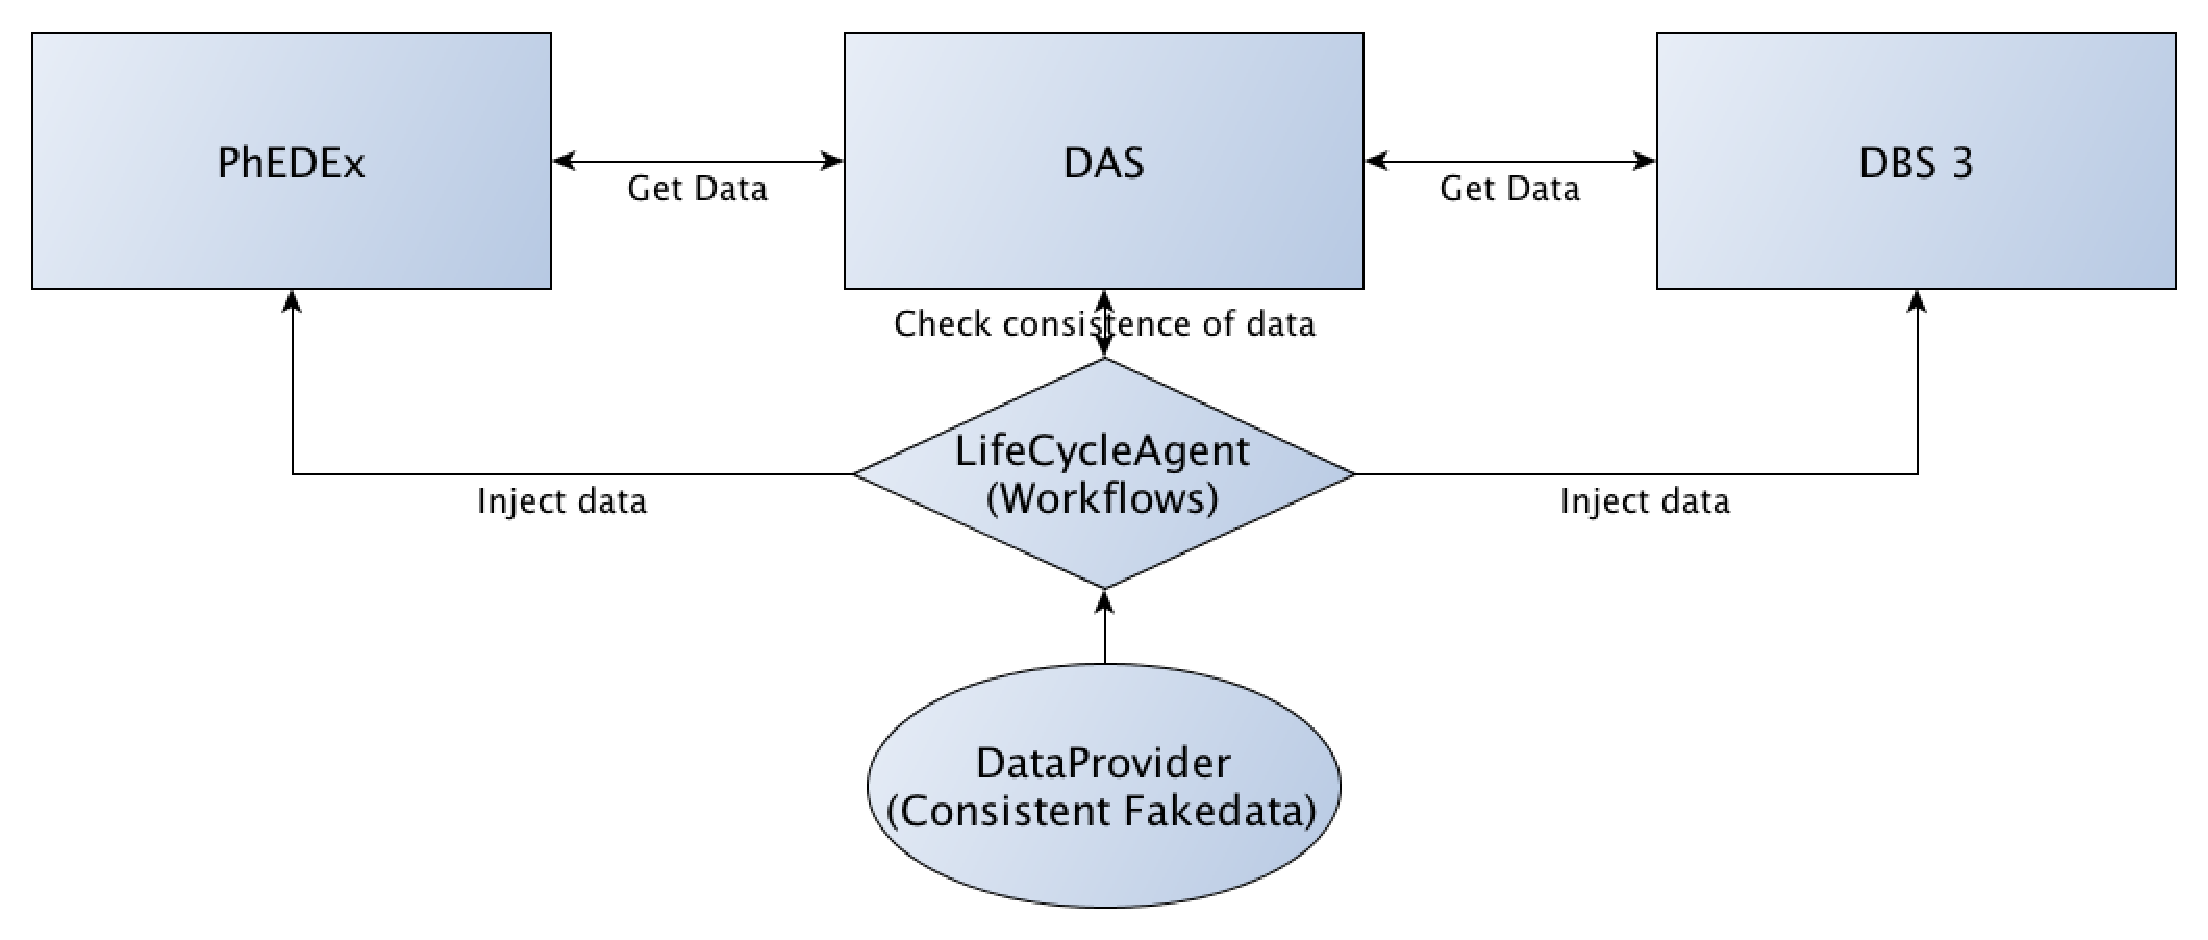
\includegraphics[width=0.8\textwidth]{IntegrationTests.pdf}
       \caption{Workflow of the integration testing of PhEDEx, DBS 3, and DAS.}
 \label{fig:Integ-Phedex-DBS-DAS}
\end{figure}

\section{Conclusions}
% placeholder...


\par
\section*{References}

\begin{thebibliography}{1}
\bibitem{CMS}
The CMS Collaboration 2008 The CMS experiment at the CERN LHC {\it JINST {\bf 3} S08004}

\bibitem{WLCG}
Knoblock J {\it et al.} 2005 LHC Computing Grid Technical Design Report {\it CERN-LHCC-2005-024}

\bibitem{OliOps}
 Gutsche O {\it et.al.} CMS Computing Operations during Run 1 {\it submitted to CHEP 2013}

\bibitem{PhEDEx}
  Egeland R, Wildish T and Metson S 2008 Data transfer infrastructure for CMS data taking,  {\it XII Advanced Computing and Analysis Techniques in Physics Research (Erice, Italy: Proceedings of Science)}

\bibitem{DBS}
Giffels M, DBS paper, {\it submitted to CHEP 2013}

\bibitem{DAS}
Kuznetsov V, Evans D and Metson S, The CMS Data Aggregation System,
{\it doi:10.1016/j.procs.2010.04.172}

\bibitem{cmscomptdr} Bonacorsi D 2007 The CMS computing model {\it Nucl. Phys.} B {\it (Proc. Suppl.)} {\bf 172} 53-56
{\bf is this a good reference or should we use the original CTDR???}

\bibitem{MongoDB}
http://www.mongodb.org/

\bibitem{MVC} Model-view-controller architecture, see
http://en.wikipedia.org/wiki/Model-view-controller

\bibitem{DASKWS} Zemleris V and Kuznetsov V,
Keyword Search over Data Service Integration for Accurate Results,
{\it submitted to CHEP 2013}

\end{thebibliography}


\end{document}

